\documentclass{beamer}
\newif\ifplacelogo
\placelogotrue
\mode<presentation>{\usetheme{Boadilla2}}

\usepackage{geometry}
\usepackage{color}
\usepackage{graphicx}

\usepackage[T1]{fontenc}
\usepackage{fontspec}
\setmainfont{CenturyGothic}
\setsansfont{CenturyGothic}

\AtBeginSection[]{\frame{\tableofcontents[currentsection]}}

\definecolor{myturquoise}{RGB}{0,176,176}
\definecolor{mylightturquoise}{RGB}{54,216,216}


\begin{document}


\setlength{\unitlength}{1mm}
\title{DS Visualisation and Analysis}
\author[Abbey Waldron]{Abbey Waldron}
\date[September 11th, 2015]{}




\setbeamertemplate{navigation symbols}{}

{
\placelogofalse
\begin{frame}
  \titlepage
\end{frame}
}



\begin{frame}{This Week - Making the right Plot!}

\begin{enumerate}
\item Show last week's work to the class
\item Introduction to making the right plot
\item Group Challenge - guess the question
\item Individual work - 2014 ebola data
\end{enumerate}

\end{frame}



\begin{frame}{Random Student Generator}

\end{frame}


\begin{frame}{Problem Set From Last Week: Irises}

\begin{enumerate}
\item Use help(iris) to understand what variables there are - make sure you know what they all mean.
\item Make a histogram (hist) with 20 bins of petal width for the Iris Setosa.
\item Make a scatterplot (tip: try ggplot2 ggplot) of sepal length vs petal length.  Show each of the three species of Iris on the same plot with a coloured legend to separate them.
\item Make a scatterplot of sepal length vs sepal width for all Irises whose petal width is greater than 1.5.
\item Make one more plot that shows something interesting about the inter-species differences of the Irises.
\end{enumerate}


\end{frame}



\begin{frame}{What does it mean to make the right plot?}


\end{frame}


\begin{frame}{What does it mean to make the right plot?}

\begin{itemize}
\item Ask a good question
\item Answer the question in one plot
\end{itemize}

\end{frame}


\begin{frame}{Practice and THINK}

\end{frame}

\begin{frame}{Calibration (normalisation)}

Same input $\rightarrow$ same output


\end{frame}


\begin{frame}{A little story}

\begin{center}
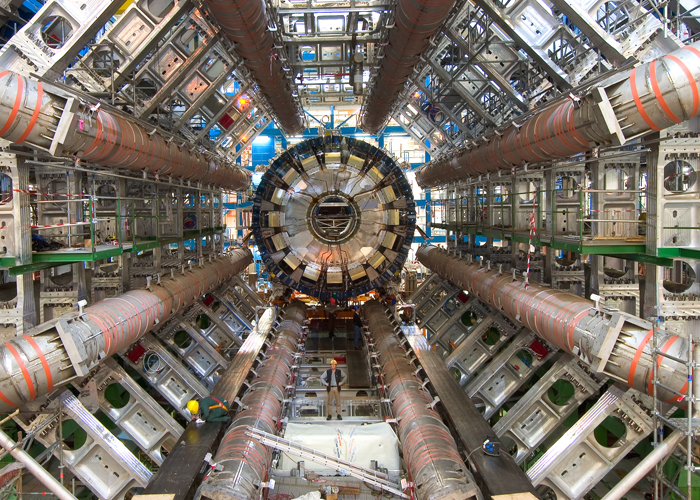
\includegraphics[scale=0.4]{pics/wk2/cern_pic.jpg}
\end{center}

demaco.nl

\end{frame}



\begin{frame}{Noise}

\begin{center}
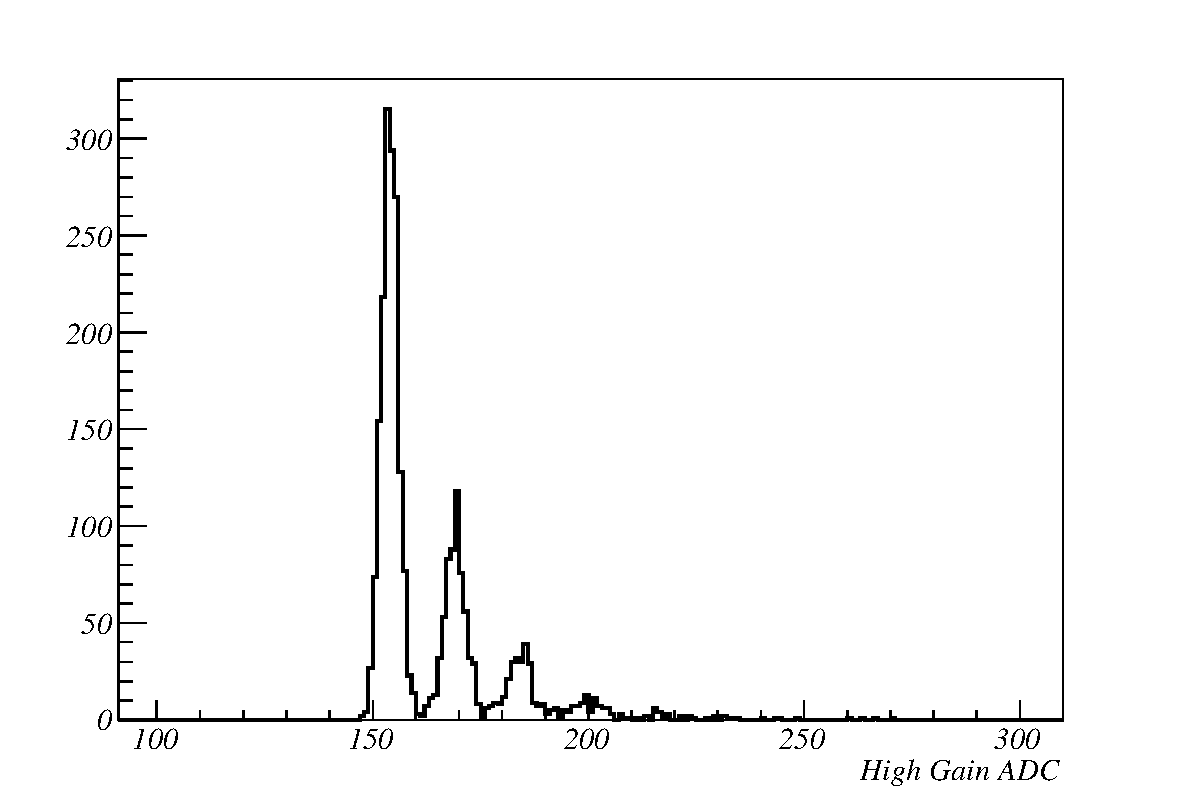
\includegraphics[scale=0.3]{pics/wk2/highped.pdf}
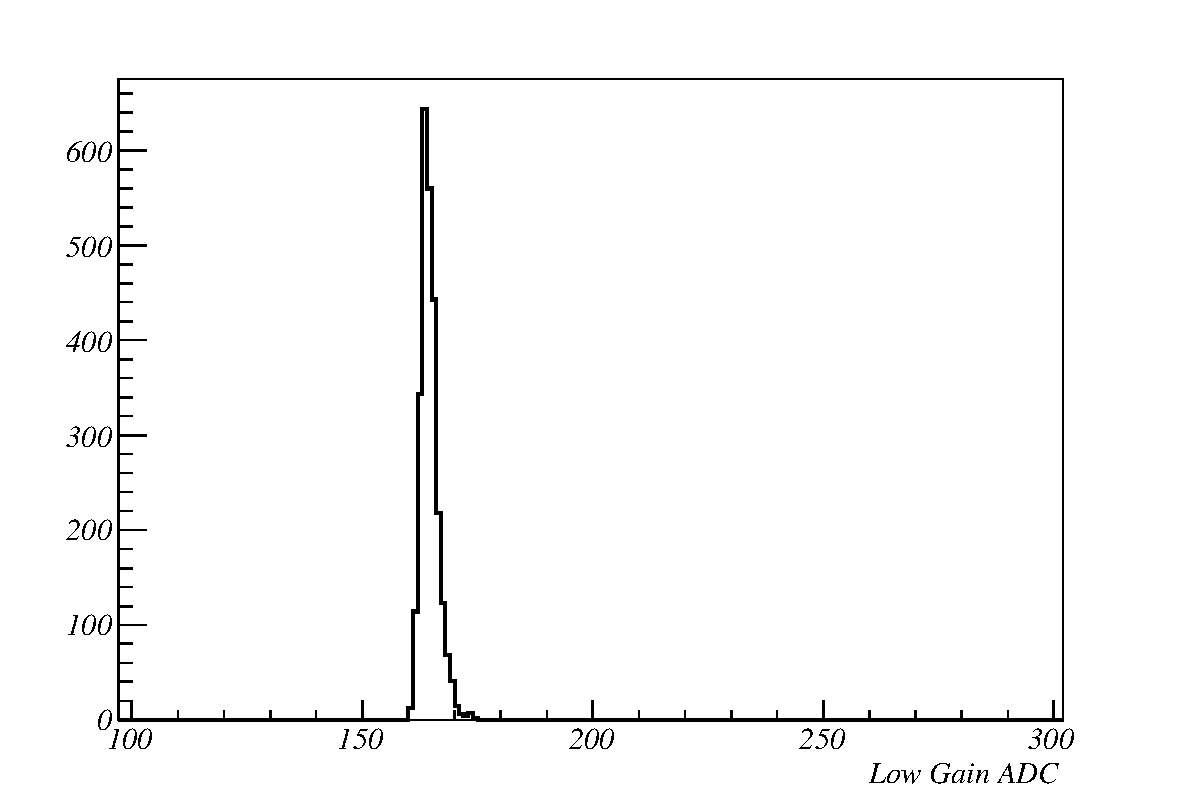
\includegraphics[scale=0.3]{pics/wk2/lowped.pdf}
\end{center}

\end{frame}


\begin{frame}{What Worked}
\begin{center}
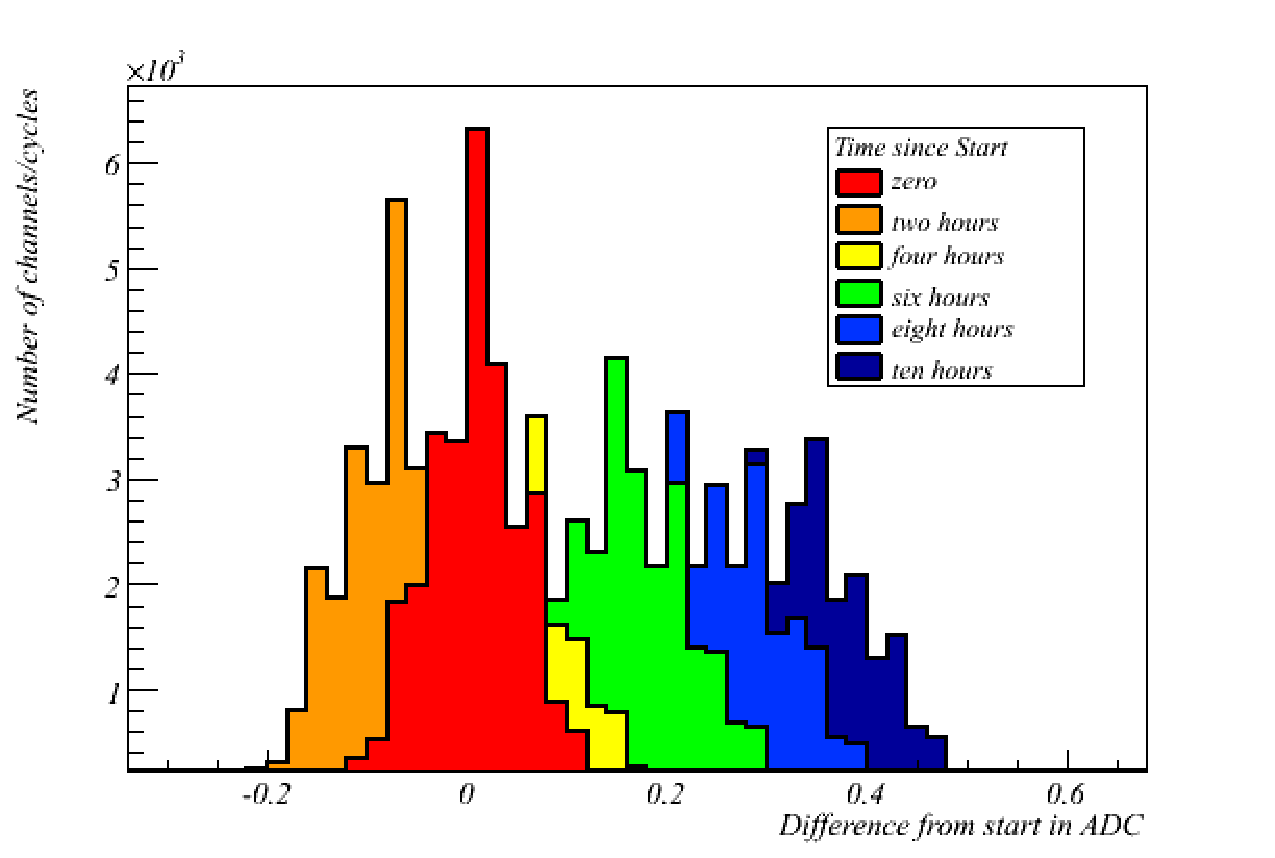
\includegraphics[scale=0.5]{pics/wk2/pedRainbow_2h.pdf}
\end{center}
\end{frame}


\begin{frame}{Group Challenge}

Here are some plots: what is the question they answer?

\end{frame}

\begin{frame}{Florence Nightingale}

\begin{center}
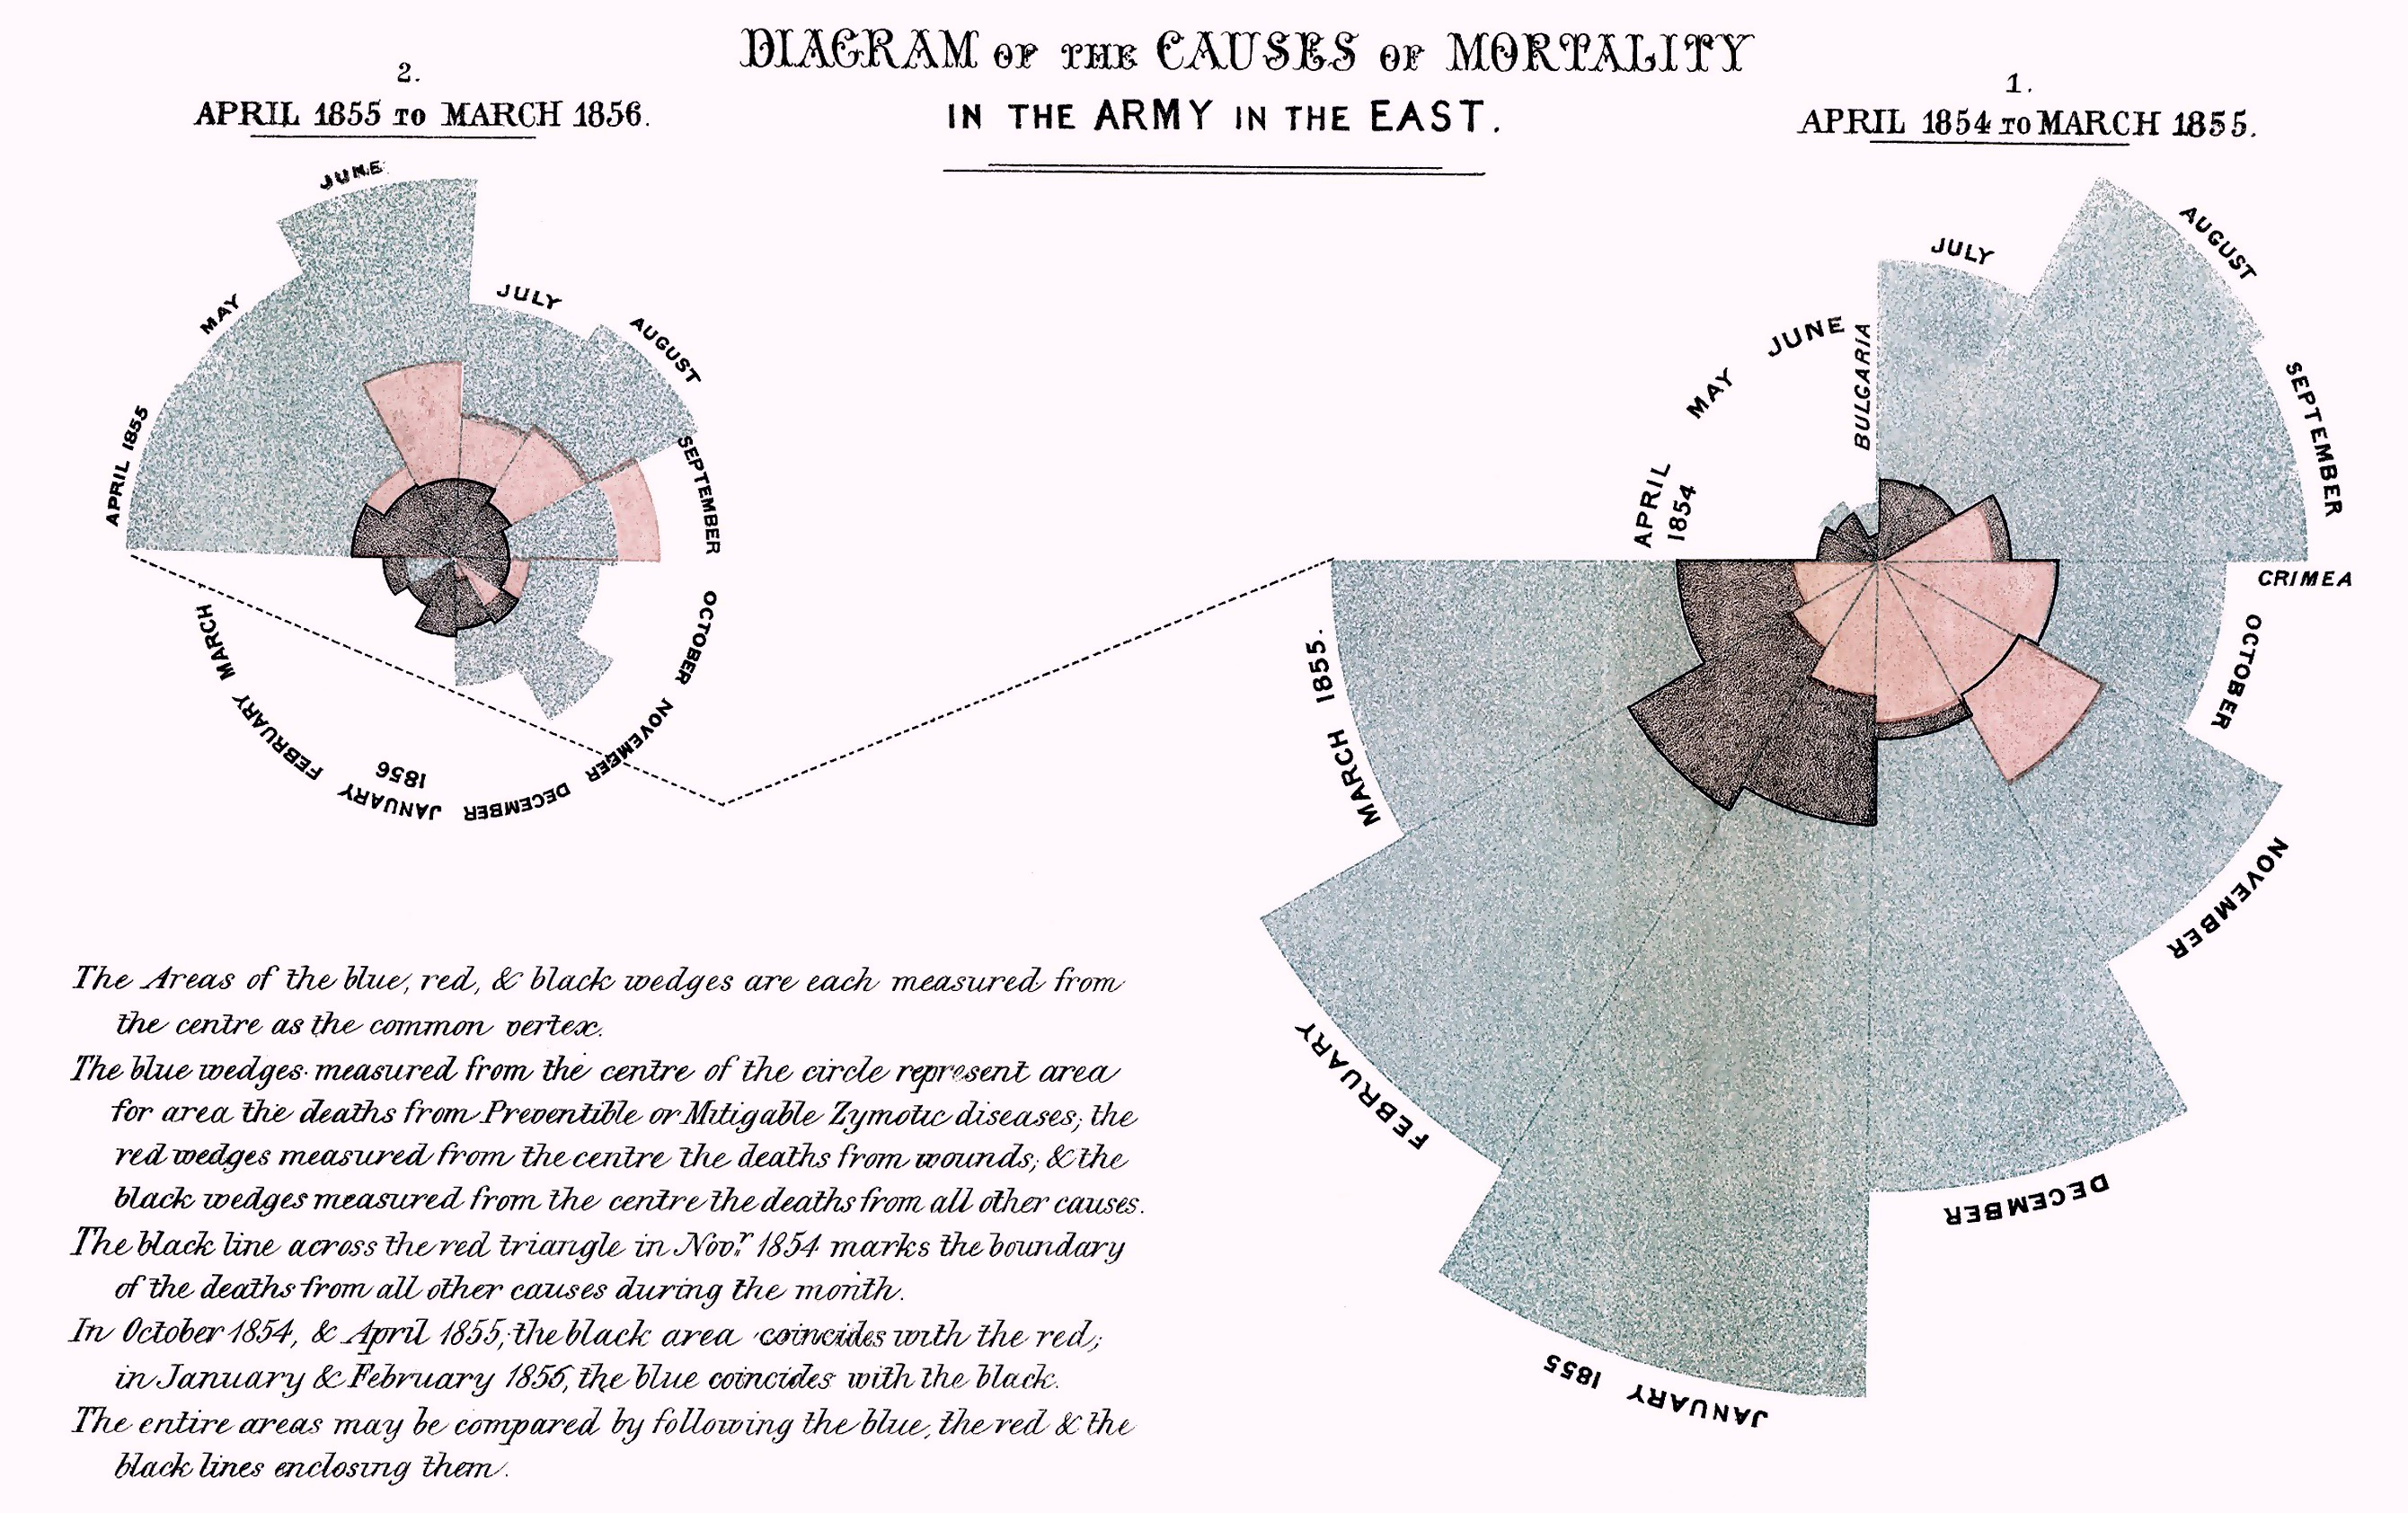
\includegraphics[scale=1.0]{pics/wk2/Nightingale-mortality.jpg}
\end{center}

\end{frame}


\begin{frame}{US Poll Results pre 2008 election}

\begin{center}
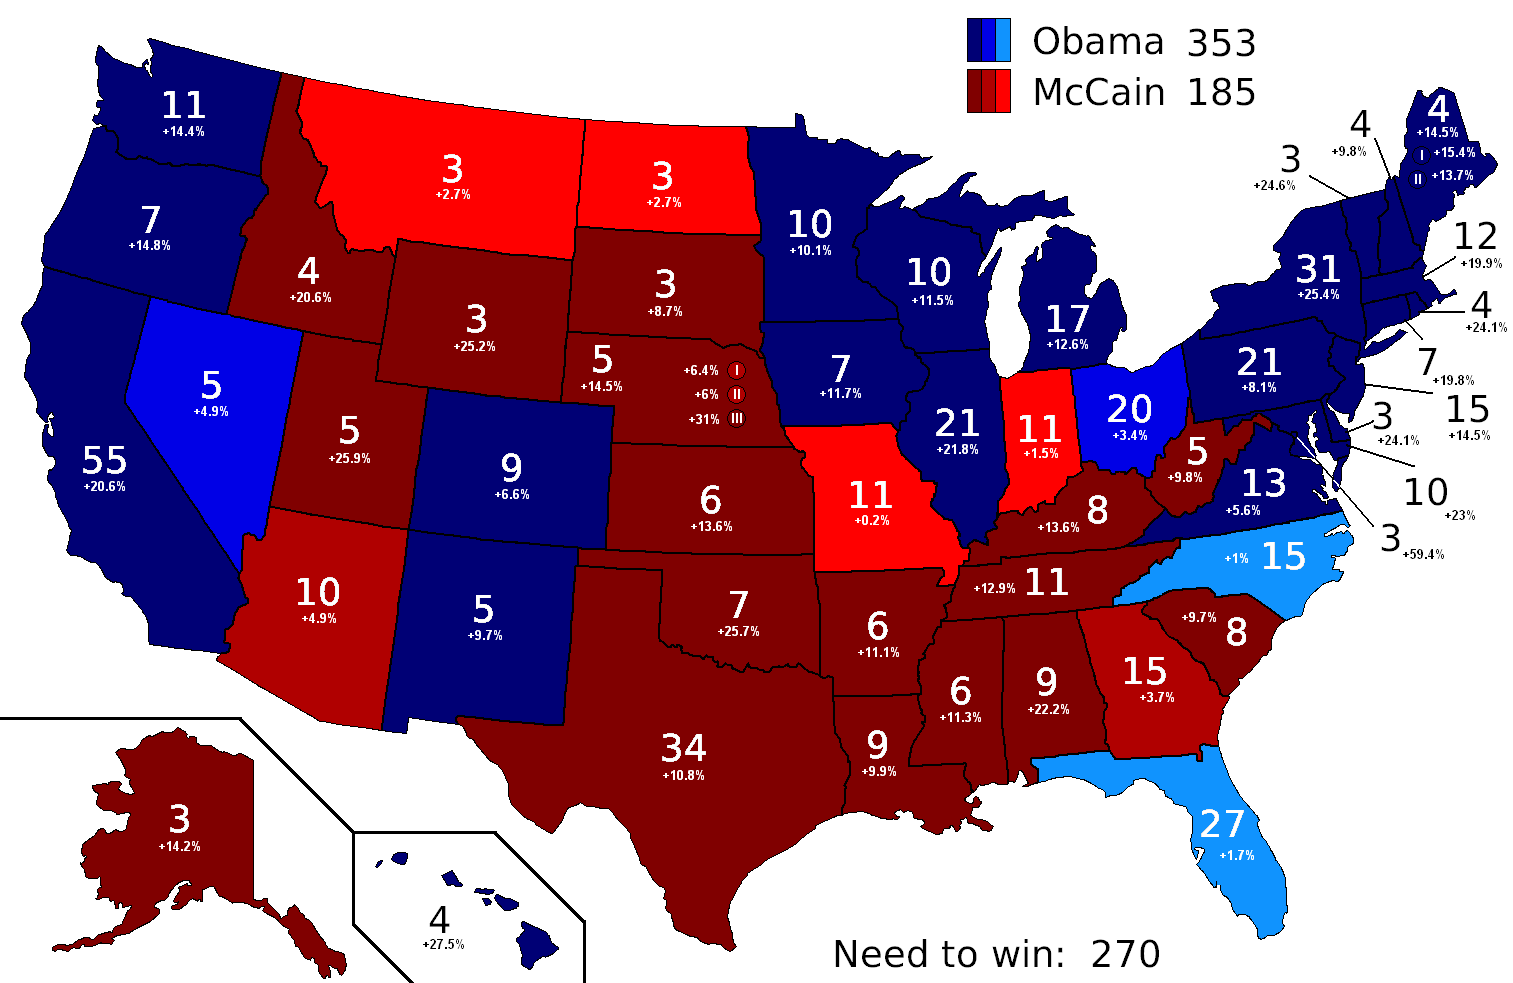
\includegraphics[scale=0.2]{pics/wk2/us_map.png}
\end{center}

Wikipedia commons

\end{frame}


\begin{frame}{Guess}

\begin{center}
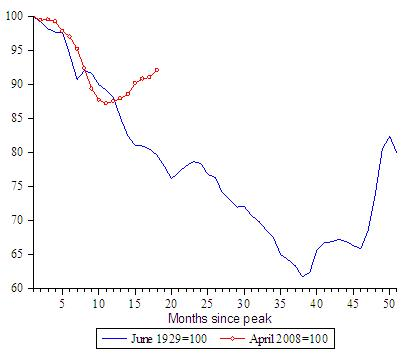
\includegraphics[scale=0.7]{pics/wk2/dep_voxeu.jpg}
\end{center}

voxeu.org

\end{frame}


\begin{frame}{This week's problems}

We will work with data from the West Africa ebola outbreak of 2013 to present.

\vspace{5mm}

Still ongoing, so far 28 000 cases are suspected to have occurred.

\end{frame}


\begin{frame}{Notes on the data}

Data is from the WHO, cite it!  The ''total'' number is only given when data of confirmed, probable and suspected cases or deaths is not known.  

\vspace{5mm}

Think carefully about which numbers you want to use for the different questions:

\begin{itemize}
\item Confirmed: laboratory tests confirm ebola
\item Probable: health workers see symptoms consistent with ebola
\item Suspected: other cases that may be ebola
\end{itemize}

\end{frame}

\begin{frame}{R Code Hints}

Some things you may need:
\begin{itemize}
\item \texttt{read.csv()}
\item \texttt{lapply}, \texttt{tapply} etc.
\end{itemize}

\vspace{5mm}

Check out the swirl stats tutorial if you don't know the last ones.

\end{frame}


%%%%%%%%%%%%% backup slides %%%%%%%%%%%%%%%%%%%%%%%%

\appendix
\newcounter{finalframe}
\setcounter{finalframe}{\value{framenumber}}

\begin{frame}{Backup Slides}
\end{frame}




\setcounter{framenumber}{\value{finalframe}}

\end{document}
